\documentclass[../main.tex]{subfiles}


\begin{document}

\section{Lecture 16}{Newton}

    \subsection{Quiz}

    \pp{1}
    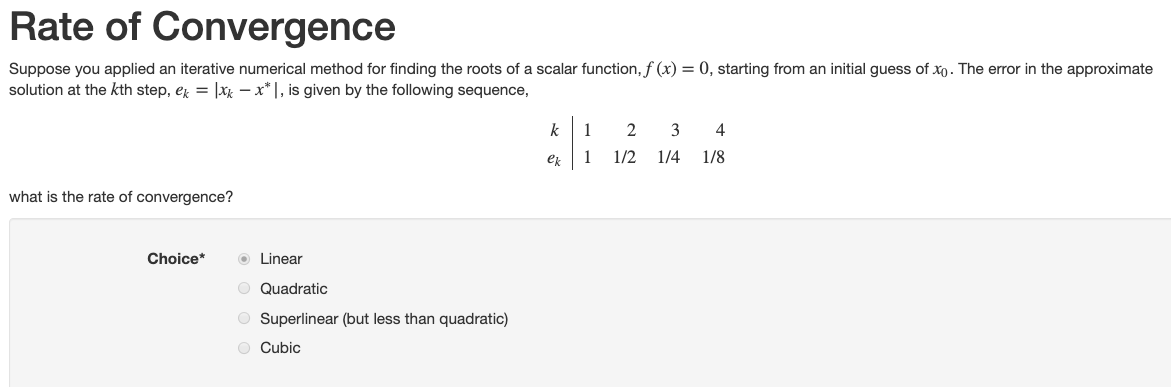
\includegraphics[width=\textwidth,height=\textheight,keepaspectratio]{lecture15q_q1}
    \begin{solution}
        The error is increasing by a constant multiplicative factor on every iteration; hence the error must be linear.
    \end{solution}

    \pp{2}
    Which of the following is true:
    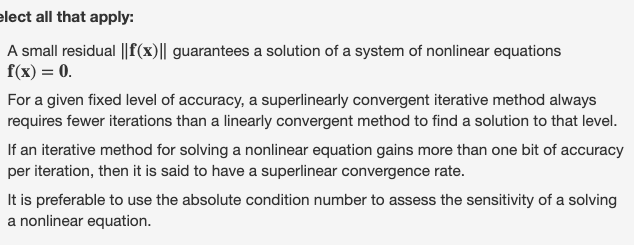
\includegraphics[width=\textwidth,height=\textheight,keepaspectratio]{lecture15q_q2}
    \begin{solution}
        A small residual may just indicate that the values of $\norm{f}$ are generally quite small. The second: if the convergence constant is above $1$, then in fact, the method will not converge -- so it really depends on the convergence constant (if the convergence constant is less than $1$ and we start off with the same initial error, the n the answer is yes). Superlinear methods need to have an increasing number of bits that they gain. In general, if the initial error is $e$ and the the convergence is rate $r$ with some constant less than $1$ as $C$ then the error at stage $m$ can be seen just by repeatedly substituting $Ce^r$ into the cheapo version of this equation and observing how the resulting value changes.
    \end{solution}

    \pp{3}
    Which value of $d$ allows us to achieve optimal convergence.
    
\includegraphics[width=\textwidth,height=\textheight,keepaspectratio]{lecture15q_q3}
    \begin{solution}
        Note that this question is a bit misleading in that we can only determine if a variant of a fixed point function is better than another variant on the basis of its behavior near a fixed point. Away from the fixed point, all bets are off. Thus, we really should be comparing, for each value of $d$, what the consequent derivative of the fixed point function $g(x) = x - f(x)/d$ is at the fixed point of the function $f$. If, however, we assume that the derivative of $g$ as $2$ sufficiently approximates the derivative of $g$ at $\sqrt{5}$ which is the fixed point that $g$ intends to navigate to, then we find that $g' = 1 - 4/d$ at $x = 2$ making $d = 4$ the best choice.
    \end{solution}

    \pp{4}
    Which value of $d$ allows us to achieve optimal convergence.
    
\includegraphics[width=\textwidth,height=\textheight,keepaspectratio]{lecture15q_q41}
    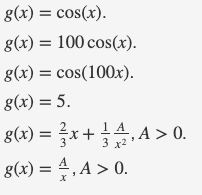
\includegraphics[width=\textwidth,height=\textheight,keepaspectratio]{lecture15q_q43}
    \begin{solution}
        The strategy is to either realize that some functions will always have a derivative at any point less than $1$ -- meaning that if the function does have a fixed point, then it will converge to the fixed point sufficiently closed to it. These functions are $g(x) = \cos(x)$ and $g(x) = 5$. Otherwise, for the remaining functions solve for $g(\xa) = \xa$ and see if $g'(\xa) < 1$. The only function that satisfies this for all values of $A$ is $g(x) = \frac{2}{3}x + \frac{1}{3}\frac{A}{x^2}$; the other $g(x,A)$ function does not; finally, I am unsure how we invalidate the functions $g(x) = 100 \cos(x)$ and $g(x) = \cos(100 x)$.
    \end{solution}

    \pp{5}
    Which value of $d$ allows us to achieve optimal convergence.
    
\includegraphics[width=\textwidth,height=\textheight,keepaspectratio]{lecture15q_q51}
    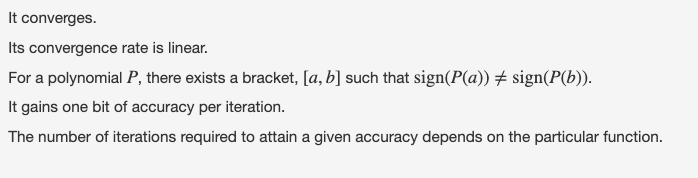
\includegraphics[width=\textwidth,height=\textheight,keepaspectratio]{lecture15q_q52}
    \begin{solution}
        Note that if we have a starting interval $[a,b]$ and we wish to reduce the error to tol, then we need to solve for the $k$ such that

        \[
            \frac{(b-a)}{2^k} = tol
        \]

        which turns out to be $\log(\frac{b-a}{tol}).$ This is true for any function.

        Note that given an interval where we've identified a root to fall into, this method always converges; its convergence is linear, because we halve the interval each time; the third remark is non-sequitur and useless; the fourth remark is true because linearly convergent methods gain a constant number of bits per iteration and here in particular, since the error goes down by a half each iteration, we gain one bit in accuracy (assuming that our interval $b-a$ is intially less than 1).
    \end{solution}

\begin{definition}
    We want to find the $h$ such that $f(x+h) = f(x) + hf'(x) = 0$. This sets $h = \frac{-f(x)}{f'(x)}$, which implies that given an initial $x_k$,

    \[
        x_{k+1} = x_k + h = x_p + \frac{-f(x_p)}{f'(x_p)}
    \]

    Set $g(x)$ to be

    \[
        x + \frac{-f(x)}{f'(x)}
    \]

    Observe that if $f'(x) = 0$ (ie if $f$ has a double root at a fixed point $x^{*}$, then $g(x^{*})$ is indeterminate and Newton fails.

    Observe that if Newton's method hits a point $y$ such that $f(y) = 0$, then $y$ is fixed point, since all successive iterates will still remain at $y$.

    Also observe that $g'(x) = \frac{f(x)f''(x)}{f'(x)^2}$ so that if $f(x) = 0$ but $f'(x) \not = 0$ (ie $x$ is a simple root), then fixed point iteration converges quadratically if we are close enough to the root -- then newton's method converges quadratically (assuming that there is no double root). Even in the event that a double root exists, it can be shown that the convergence is then linear with constant $C = 1 - 1/m$ where $m$ is the multiplicit of the root.
\end{definition}

\begin{remark}
    There are two downsides to using Newton's method:

    \begin{outline}
        \1 We need the derivative.
        \1 If we want other roots, we need to hope that some choice of another initial vector will converge to root different than the one we first found.
    \end{outline}
\end{remark}

\begin{remark}
    It is claimed that even if newton is not quadratically convergent, then it is at least linearly convergent since the derivative of the fixed point function $g'(x) = \frac{f(x)f''(x)}{f'(x)^2}$ is such that $f(x)f''(x) \to 0$ faster than $f'(x) \to 0$. Why this is true is unresolved. Indeed, Heath on page 251 explains that Newton's method is convergent with linear rate $1 - 1/m$ where $m$ is the multiplicity of the root for $m \geq 2$. It is claimed that $f(x) \to 0$. Newton breaks down in the event that the derivative function does not approximate a function very well or if  the derivative function change sign often, taking us ``left'' and ``right'' of the roots repeatedly.
\end{remark}


\begin{definition}
    The secant method works by replacing $f'(x)$ in Newton's method with $s = f(x_k) - f(x_{k-1})$. We can also use a quadratic interpolant. What does this mean?
    Recall that we approximated $f(x+h)$ by $f(x) + hf'(x)$. We could have also approximated $f(x+h)$ by $f(x) + hf'(x) + h^2f''(x)/2$. Then we need to approximate $f'(x)$ and $f''(x)$ using three points (can you guess what we might do?). Alternatively, we find an inverse quadratic interpolant that takes three points $(x,f(x)), (y, f(y)), (z, f(z))$ and then finds an inverse interpolant $q$ such that $q(f(x_i)) = x_i$. Having found this interpolant, we then let the next point be $q(0)$, since we expect that $f(q(0)) = 0$.
\end{definition}


\begin{remark}
    Both the use of newton's method through a quadratic interpolant and inverse quadratic iteration converge with superlinear rate $r \approx 1.81$.
\end{remark}

\begin{remark}
    Safeguarded methods combine several numerical methods together; for example:

    Suppose that we apply newton's method within a bracket (that is, we are given an input that falls in some set $S$). If it happens that $x_{k+1} \not \in S$, then we apply bisection and return the midpoint of the half that bisection concludes that we should use. If it does converge, then use Newton's iterate as the solution.


\end{remark}

\section{Lecture 17}

\begin{remark}
    Newton's method performs poorly if there are multiple roots.
\end{remark}

\begin{definition}
    In $n$ dimensions, fixed point iteration generalizes as follows:

    \begin{outline}
        \1 Suppose that $g: \R^n \to \R^n$. Then if $p(J(g(x^{*}))) < 1$, $g$ converges to its fixed point $\xa$ linearly. Note that $p$ is the spectral radius.
        \1 If $J(g(\xa)) = 0$, then $g$ converges to $\xa$ quadratically.
    \end{outline}
\end{definition}

\begin{remark}
    Bisection is hard to generalize for even if we could recursively find good bounds for a function $f_1$ where $f = \left[ f_1 \dots f_n \right]$, bounds particular to $f_1$ are likely unrelated to the bounds needed for $f_2$.
\end{remark}

\begin{definition}
   We can approximate $f: \R^n \to \R^n$ as 

   \[
       f(x+h) = f(x) + J(f(x))h + O(h^2)
   \]

   solving for $h$ we find

   \[
       h = -\inv{J(f(x))}f(x)
   \]

   meaning that the new iteration scheme is:

   \[
       x_{k+1} = x_{k} -\inv{J(f(x))}f(x) \tag{\alpha}
   \]
\end{definition}

\begin{remark}
    This has a couple of downsides; namely, computing the Jacobian may be expensive; moreover, computing the inverse may be expensive; finally this is only locally convergent (as before).
\end{remark}

\begin{remark}
    UNRESOLVED: when is this method quadratically convergent?
\end{remark}

\begin{remark}
    The secant method is hard to generalize, because it is not clear how we can obtain an approximation to the Jacobian $J(f(x))$ using only $f(x_1), f(x_2), x_1, x_2$ although obtaining an approximation to $f'(x)$ given $f(x_i)$ and $x_i$ is certainly plausible. Broyden's method starts with a guess for $J(f(x))$, and then with some update akin to $(\alpha)$it then finds the next Jacobian.
\end{remark}

\subsection{Optimization}

\begin{lemma}
    If a function is continuous on a closed and bounded set $S \s \R^n$, then it attains its minimum and maximum. See \url{https://en.wikipedia.org/wiki/Extreme_value_theorem#Proof_of_the_extreme_value_theorem} for the proof.
\end{lemma}

\begin{definition}
    A function is coercive if $\lim_{\norm{x} \to \infty} f(x) = \infty$. A coercive function attains a global minimum, although the minimum may not be unique. Think of a cubic function with two dips.
\end{definition}


\begin{definition}
    A set $S$ is convex if for $x,y \in S$ it holds that $x(\alpha) + y(1 - \alpha) \in S$ for all $\alpha \in [0,1]$. A function $f$ is convex if it holds that $f(x \alpha + y (1 - \alpha)) \leq \alpha f(x) + (1 - \alpha)f(y)$. 
\end{definition}

\begin{proposition}
    If a function $f$ is continuous and convex, then it attains a minimum; if it is instead strictly convex and continuous, then its minimum is unique.
\end{proposition}

\begin{lemma}
    The following are sufficient and necessary conditions for minimality in $1$ dimension and in $\R^n$.
    \begin{outline}
    \1 $\R^1:$ 
    \2 $f'(x) = 0$ is a necessary condition.
    \2 In conjunciton with $f''(x) > 0$, the foregoing is a sufficient condition.
    \2 $\nabla f(x) = 0$ is a necessary condition.
    \2 In conjunction with $H(f(x)) > 0$ -- ie the Hessian being positive definite -- we get a sufficient condition.
    \end{outline}
\end{lemma}

\begin{definition}
    A  matrix admits a Cholesky Decomposition, a factorization of the form $LL^{*}$ where $L$ is lower triangular, iff it is positive definite hermitian. In particular, if $A$ is positive definite, then the factorization is unique; but if $A$ is merely positive semidefinite, then the factorization is not unique; if $A$ is not event positive semidefinite, then the cholesky decomposition will have a negative entry somewhere along the diagonal (this is not true otherwise).
\end{definition}

\begin{remark}
    We can find the minimum of a function $f$ by solving for $\nabla f = 0$ using any of the methods that we've developed for multidimensional root finding. To then assert that the found root actually corresponds to a minimum, we need to check whether the Hessian of the matrix is positive definite. Note that since $H$ is symmetric, if we attempt to decompose $H$ into a Cholesky Decomposition and find that it has a negative entry on one of its diagonals, then the matrix is in fact not positive definite. 
\end{remark}

\begin{proposition}
    The error in a solution to an optimization problem is at best $10^{-8}$.
\end{proposition}

\begin{proof}
    Suppose that $\xa$ is a true minimizer but that we estimate $\hat{x}$ to be the minimizer instead. Let $\hat{x} = \xa + h$. Then observe that

    \[
    f(\xa + h) \approx f(\xa) + f'(\xa)h + f''(\xa)h^2/2 = f(\xa) + f''(\xa)h^2/2 \implies h^2 = \frac{2(f(\xa + h) - f(\xa))}{f''(\xa)}
    \]

    What this implies is that if we take $\hat{x}$ to be a solution and we have $\abs{f(\hat{x} - f(\xa)} < \e$, then our error in $\hat{x}$, which is $h$, is at best $\sqrt{\frac{2\e}{f''(\xa)}}$. This is about $10^{-8}$, implying $8$ accurate digits, if $\e = \e_{mach}$. We upper bounded the error in $\xa$, which suggests that we should revise our original statement to be that we can at least get a tolerance of $10^{-8}$. The fact that during the course of a problem, we can conceivably find $\hat{x}$ such that $\abs{\hat{x} - \xa} \approx \e_{mach}$ and declare this value our minimum makes this a best bound however.
\end{proof}

\begin{remark}
    The follwoing facts about convexity should be known:

    \begin{outline}
        \1 If a convex function has a local minimum, then the local minimum is, in fact, a global minimum.
        \1 If a strictly convex function has a local minimum, then the local minimum is a unique global minimum.
        \1 If a continuous function is restricted to a closed and bounded set $S \s \R^n$, then $f(S) \s \R$ is compact and, hence, obtains a minimum, so that there is a minimum $x \in S$ of $f$.
        \1 More generally, if $f$ is a continuous function restricted to a closed but unbounded set and $f$ is coercive, then $f$ attains a minimum. This can be proven. Note that a convex function on a convex set is necessarily continuous at interior points of its domain. This has never been proven.
    \end{outline}
\end{remark}
\section{Lecture 18}

\subsection{Quiz}

\pp{1}
Comparison of Newton and Broyden Methods
Which of the following is NOT an advantage of Broyden's method over Newton's method for solving a system of nonlinear equations?
Choice*
Matrix factorization can be updated each iteration rather than having to be recomputed
No derivatives required
Less work per iteration
Fewer iterations required for given accuracy

\begin{solution}
    Matrix factorization has to be updated in Newton's method everytime -- meaning that
    we have to compute the Jacobian every time. The Jacobian method also requires a Jacobian
    which is not required by Broyden's method. The update in Broyden's method also resembles
    a Sherman-Morrison update, making it less costly per iteration to compute the next Jacobian (approximation to the Jacobian) than in Newton's method (this is true in spite of the fact
    that Broyden's method also computes a difference of the form $f(x_{k+1}) - f(x_{k})$.
\begin{center}
    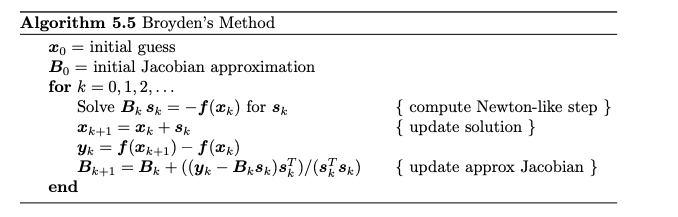
\includegraphics[width=\textwidth,height=\textheight,keepaspectratio]{lecture17_broyden}
\end{center}
\end{solution}

\pp{2}

Easy to tell what a convex set looks like.

\pp{3}

Have to review convexity.

\pp{4}

Simply remember that the Hessian is the transpose of the Jacobian of the gradient. ALso remember that if a hessian is neither positive semidefinite nor negative semidefinite at a point where the gradient is zero, then the critical point is a saddle point. 

\pp{5}
Optimization Accuracy
Suppose that f can be evaluated to within a relative error of 10−10. If x∗ is an extreme point of f, with $\abs{f''(x)} = 1$, then about how many decimal digits of x∗ can reliably be computed as a solution to an optimization problem?

\begin{solution}
    Apply the lemma. from the previous lecture.
\end{solution}

\begin{definition}
\begin{center}
    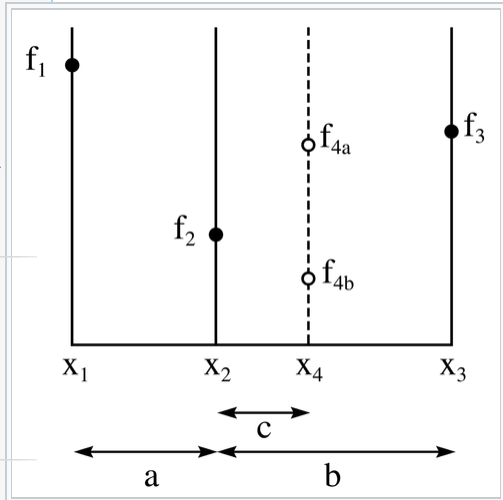
\includegraphics[width=\textwidth,height=\textheight,keepaspectratio]{lecture18_golden_search}
\end{center}

In golden section search,  given an interval $[x_1 , x_3]$ (or in our case the interval is often denoted $[a,b]$) we choose points inside the interval $x_2, x_4$ (in our case, we define these points to be $a + (b - a)(1 - \tau)$ and $a + (b - a)\tau$ such that

\[
    \frac{\abs{x_3 - x_2}}{\abs{x_2 - x_1}} = \frac{\abs{x_2 - x_1}}{\abs{x_4 - x_2}}
\]

In the diagram above, we see that at any point in the initiation of a golden search we have three points that are known, and depending on the function evaluation of the fourth point, we will choose the subinterval $[x_1, x_4]$ or $[x_2, x_3]$.Thus the stipulation that $c/a = a/b$ represents our desire that when we recurse into a new subinterval that the three given points have been some subset of the givens and function evaluations in the interval ``one frame up.'' Note that this inequality assumes that we progress into the left subinterval; the analysis for the right subinterval is the same, however, since $a + c = b$ and $b -c = a$ (that is $\abs{x_3 - x_4} = \abs{x_2 - x_1}$

It can be shown that solving this proportion requires that $\tau$ be the golden ratio.


    
\end{definition}
\begin{definition}
    Newton's method for optimization is to use newton's method for root finding in order to solve $f'(x) = 0$. We explore the 1-D case, because this easily generalizes to the n-D case:

    \begin{align*}
        f(x + h) = hf'(x) + h^2 f''(x)/2 + O(h^3) \\
        \intertext{Differentiate this with respect to $h$}: \\
        f'(x + h) = f'(x) + h f''(x) + O(h^3) \\
        \intertext{Set this to $0$ and solve for $h$} \\
        h = \frac{-f'(x)}{f''(x)} \\
        \intertext{So the update becomes} \\
        x \leftarrow x - \frac{f'(x)}{f''(x)} \\
        \intertext{In n-D, this will generalize to:} \\
        \mathbb{x} \leftarrow \mathbb{x} - \inv{(H_f(x))}\nabla f(x) \tag{$\beta$}\\
    \end{align*}

    This quadratic approximation of $f$ via a taylor series expansion is only accurate within a region. If we define what that region us as a ball centered at $x$with radius $r$ and we see that $r < \abs{\inv{(H_f(x))}\nabla f(x)}$ then we can bind the decrement to be precisely $r * \inv{(H_f(x))}\nabla f(x)/\abs{\inv{(H_f(x))}\nabla f(x)}$.

    For reasons that are not clear, this approach (called using a trust region), may also change the direction of the search. Note that we can also employ a so called line search to find the scalar factor of $\inv{(H_f(x))}\nabla f(x)/\abs{\inv{(H_f(x))}\nabla f(x)}$ that best minimizes $(\beta)$.
\end{definition}


\begin{definition}
    Gradient descent repeatedly runs the following function

    \[
        \mathbb{x_{k+1}} \leftarrow \mathbb{x_{k}} - \alpha_k \nabla f(x_k)
    \]

    where $\alpha_k$ is chosen using some other method. For example. One may try to optimize the function $g(\alpha_k) = \mathbb{x_{k}} - \alpha_k \nabla f(x_k)$.

\begin{center}
    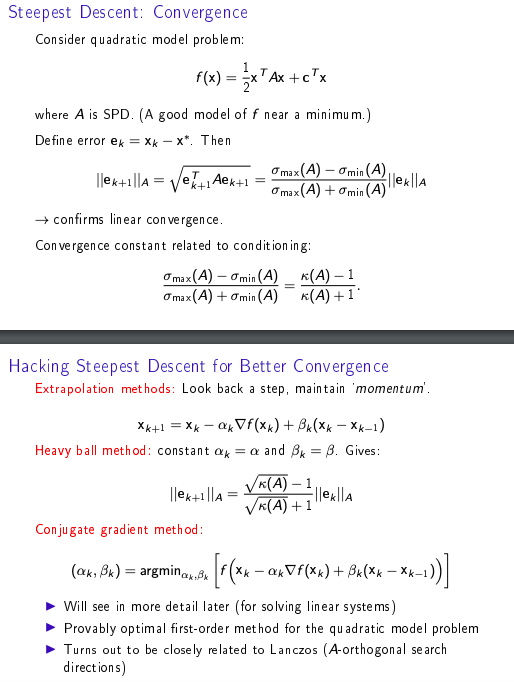
\includegraphics[width=\textwidth,height=\textheight,keepaspectratio]{lecture18_steepest_rates}
\end{center}
\end{definition}


\section{Lecture 19}

\subsection{Quiz}
\pp{1}
Unimodal Function
Suppose the real-valued function f(x) is unimodal on the interval [a,b]. Let x1 and x2 be two points in the interval, with a<x1<x2<b. If f(x1)=1.232 and f(x2)=3.576, then which of the following statements is valid on the subinterval [a,b].

\begin{solution}
    Recall that unimodality tells us that if we have two points $x$ and $y$ such that $a \leq x < y \leq b$ and $f(x) < f(y)$ then the minimum will be found going ``down the slope'', meaning that it will be contained in the interval $[a,y]$. Then tells us that the solution is that the minimum must lie in the interval $[a, x_2]$. There is an option that attempts to dupe us: The subinterval of the minimum of $f$ is indeterminate without knowing the values of $f(a)$ and $f(b)$. This is not true, however -- if we are granted unimodality on $[a,b]$ even without knowing the values of $a$ and $b$ we can be assured of the statements in this solution.
\end{solution}

\pp{2}
Golden Section Search
Suppose we decided to use golden section search for finding the minimum of a unimodal function, but, in the inner loop of the algorithm, instead of picking evaluation points x1,x2 using the formulas

x1=a+(1−τ)(b−a)
x2=a+τ(b−a)
at each iteration (where a and b are the endpoints of the interval, and τ=12(5‾√−1)), we chose

x1=a+13(b−a)
x2=a+23(b−a).
The remainder of the algorithm is the same. This modified strategy is called ternary search.

What is a legitimate disadvantage of using ternary search compared to golden section search?

\begin{solution}
    These were the choices:

    On average per iteration, ternary search necessarily requires evaluating the function at more points.
There are no substantial disadvantages compared to golden section search.
The convergence rate of ternary search may be sublinear, while that of golden section search is always linear.
Ternary search may fail to converge for some unimodal functions for which golden section search converges.

    If we use ternary search, then we don't preserve the proportion that we listed above, requiring us to have on more function evaluation. Note that with ternary search, the interval length shortens by $2/3$ every time. Note that because unimodality is always preserved and the interval decreases, ternary search must converge.
    Thus, the answer is the first choice.
    
\end{solution}

\pp{3}
Robust Newton Methods
For unconstrained optimization of a function f:ℝn→ℝ, Newton's method is often unreliable when started far from the solution. How do line searches or trust regions improve its reliability?

Select all that apply:
A trust region modifies the length of the Newton step.
A line search modifies the length of the Newton step.
A line search modifies the direction of the Newton step.
A trust region modifies the direction of the Newton step.

\begin{solution}
    See the logic above. The following are true:
A trust region modifies the length of the Newton step.
A line search modifies the length of the Newton step.
A trust region modifies the direction of the Newton step.
\end{solution}

\pp{4}
Convergence Rates
Recall the definition of convergence rates

limk→∞‖ek+1‖‖ek‖r=C
We are trying to minimize

$f(x)=\frac{1}{2} x^T \begin{bmatrix}
    4 & 0 \\
    0 & 3 \\
\end{bmatrix}x$
If we are using steepest descent to minimize f, what is r and C? Give 4 significant figures.

\begin{solution}
    See the page on convergence rates in the your notes from the previous lecture.
\end{solution}


\pp{5}
Newton's Method
Consider minimization of the function
$ϕ(x,y)=(x−2)^2+(y−1)^2$
Starting with an initial guess [x,y]0:=[0,0], what are the values of x and y after one round of Newton's Method

\begin{solution}
    Compute the gradient; compute the hessian $A = H_f(0,0)$

    Then solve for

    \[
        A(s_k) = - \nabla f(0,0)
    \]
\end{solution}

\begin{definition}
    Newton's method in $N$ dimensions does the following:

    \begin{align*}
        f(x + h) = f(x) + \nabla f(x) h + \frac{1}{2} h^T H_{f}(x) h \\
        \intertext{Now differentiate with respect to $h$ and solve for $h$} \\
        0 =  \nabla f(x) + H_{f}(x) h \\
        \intertext{Then set $x_k \leftarrow x_k + h$ } \\
    \end{align*}
\end{definition}

\begin{remark}
    This method has a few problems:

    \begin{outline}
        \1 It depends on the validity of a Taylor expansion and, hence, is only 
        locally convergent.
        \1 It requires that we compute second derivatives.
        \1 UNRESOLVED (works poorly when $H_f$ is nearly indefinite).
    \end{outline}
\end{remark}


\begin{definition}


\begin{center}
    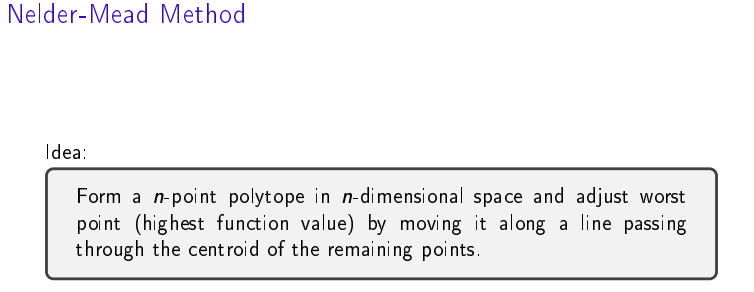
\includegraphics[width=\textwidth,height=\textheight,keepaspectratio]{lecture19_nelder_mead}
\end{center}

\end{definition}

\begin{definition}
    Let $y - a(x) = r(x)$ and suppose that we wish to minimize

    \[
        \phi(x) = \frac{1}{2}r(x)^Tr(x) = \frac{1}{2}\sum_{i=1}^{n}r_i(x)^2
    \]

    \[
    \frac{\partial}{\partial x_i}\phi(x) = \sum_{j=1}^{n} \frac{\partial r_j(x)}{ \partial x_i }(r_j(x)) \implies \nabla \phi(x) = J^T(x) r(x)
    \]

    This then gives:
    \[
        \frac{\partial^2}{\partial x_k \partial x_i}\phi(x) = \sum_{j=1}^{n} \frac{\partial^2 r_j(x)}{ \partial x_k \partial x_i }r_j(x) + \frac{\partial r_j(x)}{\partial x_i}  \frac{\partial r_j(x)}{\partial x_k} \implies H_{\phi}(x) = J^TJ + \sum_{j=1}^{n}r_{j} H_{r_{j}}(x)
    \]


    We assume that the terms $r_j H_{r_j}(x) \approx 0$ so that $H_{\phi}(x) = J^TJ$. Then the step size in newton's method, $- \inv{H_{\phi}(x)} \nabla \phi(x)$ becomes $- \inv{(J^TJ)}J^Tr(x)$. \\


    That is, Gauss Newton computes the step size by computing $s$ where $J(x)s \approx r(x)$

\end{definition}
\section{Lecture 20}

\subsection{Quiz}


\pp{1}

We use the approximation

\[
    x_k \leftarrow x_{k-1} + \alpha \inv{(H_{f}(x))} (-\nabla_{f}(x))
\]

\begin{align*}
    \intertext{This works out to be} \\
    x_k \leftarrow 
    [2, 1]^T + 1 \begin{bmatrix}
        1 & -0.5 \\
        0 & 1 \\
    \end{bmatrix} (- \begin{bmatrix}
        \cos(x_1) \\
        -\sin(x_2) \\
    \end{bmatrix}) \\
    \intertext{Let us approximate $\cos(x_1) = \cos(2)$ by $-0.41614$ and let us approximate $-\sin(x_2) = -\sin(1)$ by $-0.84147$. This gives us} \\ 
    [2, 1]^T + \begin{bmatrix}
        1 & -0.5 \\
        0 & 1 \\
    \end{bmatrix}^{-1} (- \begin{bmatrix}
        -0.41614 \\
        -0.84147 \\
    \end{bmatrix}) \\
\end{align*}

See the code below
    %>>> A
    %array([[ 1. , -0.5],
    %[ 0. ,  1. ]])
    %>>> np.linalg.inv(A) @b * -1  + np.asarray([2,1])

\pp{2}
Secant Updating Methods
For unconstrained minimization of a function f:ℝn→ℝ, why is it not a good idea to find a critical point by using Broyden's method to solve the nonlinear system ∇f(x)=0?
Select all that apply:
It would require a matrix factorization at each iteration.
It would not preserve symmetry of the approximate Hessian matrix.
It would require evaluation of the Hessian matrix.
It would not converge superlinearly.

\begin{solution}
    First recall what Broyden's method is. Brodyen's method computes the solution to $\nabla_{f}(x) = 0$ using a series of approximations. We start with an initial approximation of the Jacobian $B_k$. Then we compute a step size that will update the current value of $x_{k+1}$. This gives us an updated value of the diference $f(x_{k+1}) - f(x_{k}) = y$. We then use $y$ and $x_{k+1}, x_{k}$ to update $B_k$ with some update resembling a Sherman Morrison update. Note taht this update is not guaranteed to preserve symmetry of the Hessian matrix. Realize that here $B_k$ corresponds to the Hessian. Secant methods have been shown to converge superlinearly, so the convergence would still be superlinear; at no point do we ever explicitly evalute the object that $B$ mocks so there is no evaluation of a Hessian or anything of that sort.
\end{solution}

\pp{3}
Gauss-Newton vs. Newton
Which of the following statements about Gauss-Newton in comparison with 'regular' Newton applied to the 2-norm of the residual norm

\[
    \phi(x) \coloneq \frac{1}{2}\norm{f(x) - y}_2^2
\]

Gauss-Newton requires fewer known derivatives.  \\
The approximation to Hϕ used by Gauss-Newton may be inaccurate if the residual is large. \\
Gauss-Newton has a lower cost per iteration. \\
The two are equivalent. \\
Gauss-Newton uses a more accurate approximation to f in computing the next iterate. \\
Both converge globally \\

\begin{solution}
    Recall that Gauss newton approximates the Hessian as $J^TJ$ and ignores the terms $r_i H_{r_i}(x)$;if the residual terms actually happen to be big, then our approximation is off. Note that since Gauss Newton does not use the Hessian explicitly, the costs of finding derviatives that are part of the Hessian are non-existent in Gauss-Newton (and so Guass newton has a lower costs per iteration).
\end{solution}

\pp{5}
Constrained Optimization
Consider the constrained optimization problem

minf(x),g(x)=0.
At a minimal point, ∇f(x) must...


\begin{solution}
    \begin{align*}
        f(x) - \lambda^T g(x) = 0 \\
        \implies J(f(x)) - J(\lambda^T g(x)) = 0 \\
        = J(f(x)) - \lambda^T J(g(x)) = 0 \\
        \implies \nabla_{f}(x) = J(g(x))^T \lambda \\
    \end{align*}
        hence only the first choice is correct.
\end{solution}



\begin{definition}
    A constrained optimization problem is of the form:

    \[
        \min f(x) \st g(x) = 0
    \]

    here $f: \R^n \to \R^1$ and $g: \R^n \to \R^m$.
\end{definition}



\begin{remark}
    Let the feasible set (ie those $x$ such that $g(x) = 0$) be $S$.
    Given a point $x \in S$, we say that a direction $s$ is feasible
    if for some $\alpha \in [0,r)$ where $r >0$ that $x + \alpha *s \in S$ as well.
    A first order condition is that at the boundary of the feasible set,
    if $s$ is a feasible direction then,

    \[
        \nabla f(\xa)^T s \geq 0
    \]

    or else, we would proceed in the direction of $s$ and hence minimize $f$.

    If we are at an interior point, then both $s$ and $-s$ are feasible directions in which csae the optimality condition implies that $\nabla f(\xa) = 0$, which coincides with the first order optimality condition for unconstrained optimization. Indeed, constrained optimization is only interesting at the boundary of the feasible set, because constrained optmization problems behave like unconstrained optmization problems at the interior of the feasible set.
\end{remark}

\begin{remark}
    A second order optimality condition is that for any point $x$ with a feasible direction $s$ it holds that

    \[
        s^T H_{f}(\xa)s \geq 0
    \]

    It is easy to see why this is a necessary condition for the unconstrained case, for an approximation to $f(\xa + s)$ is given by

    \[
        \nabla f(\xa) \cdot s + s^T H_{f}(\xa)s
    \]

    so that if $s^T H_{f}(\xa)s< 0$, then $f(\xa + s) < f(\xa)$, contradicting that $f(\xa)$ is optimal. It is not clear, however, why this is a necessary condition for a boundary point, for it may just take place that in the approximation above of $f(x + a)$, if $\nabla f(\xa) \cdot s > \abs{s^TH_{f}(\xa)s}$, then $f(\xa + s) > f(\xa)$.
\end{remark}

\begin{proposition}
    At an optimal point $\xa$, it holds that

    \[
        - \nabla f(\xa) = J_{g}^T \lambda^{\ast}
    \]

    for some $\lambda^{\ast} \in \R^m$.
\end{proposition}

\begin{proof}
    This is easiest to imagine:
\begin{center}
    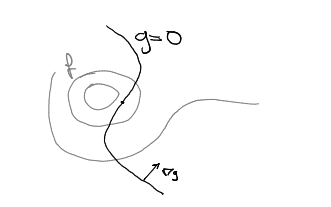
\includegraphics[width=\textwidth,height=\textheight,keepaspectratio]{lecture20_langrange}
\end{center}

Suppose that the dotted point is $\xa$. Now if we try to proceed in the direction of greatest descent, which is $- \nabla f(\xa)$, then we find that we must move in the direction of greatest ascent for $g$. That is, any further attempt to minimize $f$ necessarily forces us to violate our constraint on $g$ and, hence, fall off of the level set $g = 0$. \\

It is known that $\nabla f(x)^T$ is the direction of greatest ascent (recall that there is some calculus proof that explains that not only does $\nabla f(x) \cdot s$ where $s$ is some $n$ vector give us the instantaneous increase in the direction $s$ but that were $s$ in the direction of $\nabla f(x)$ itself, we would increase most rapidly (indeed use the cosine identity involving the dot product). One can similarly generalize (though, I am not sure how) and conclude that $(\nabla g)^T = J_{g}^T$ gives us the direction of greatest ascent in $g$. \\

We hit $J_{g}^T$ by some $m$ vector to give us an $n$ vector.
\end{proof}

\begin{definition}
    The lagrange function is defined to be

    \[
        L(x, \lambda) f(x) + \lambda^T g(x)
    \]

    since then $\nabla L = 0 \implies \nabla f(x) + J_{g}(x)^T \lambda = 0$ and $g(x) = 0$. That is

    \[
        \nabla L = 
        \begin{bmatrix}
            \nabla_{x} L(x, \lambda) \\
            \nabla_{\lambda} L(x, \lambda)
        \end{bmatrix} = 
        \begin{bmatrix}
            \nabla f(x) + \lambda^T g(x) \\
            g(x)
        \end{bmatrix}
    \]

    which are necessary conditions that we previously discussed.

\end{definition}


\begin{remark}
    If we wish to compute the hessian of this function, then simply do the following, take the jacobian with respect to $x$ of the first row of $\nabla L$ and with respect to $\lambda$ of first row; the resulting entries become the first row of the Hessian; likewise, obtain the second row of the Hessian. This gives us

    \[
        H_{L}(x, \lambda) = \begin{bmatrix}
            B(x, \lambda) & J_{g}^T x \\
            J_{g}(x) & 0
        \end{bmatrix}
    \]

    where $B(x, \lambda) = H_{f}(x) + \sum_{i=1}^{m}\lambda_{i} H_{g_i}(x)$.

    Note that since a matrix is positive definite if and only if its eigenvalues are all positive, and the product of the diagonals of a matrix is the product of its eigenvalues, $H_{L}$ is not positive definite (since it has $0$ as an eigenvalue). This matrix is, however, symmetric (check this yourself).
\end{remark}


\begin{remark}
    As a consequence, Heath asserts that any critical point of the Lagrangian is necessarily a saddle point. That is, it must hold that at $\xa$, there exists $s_1$ such that $s_1^TH_{f}(\xa)s_1 > 0$ and $s_2$ such that $s_2^TH_{f}(\xa)s_2 < 0$. UNRESOLVED (Why is this true?) At present, the only lead I have is that if, suppose, that $\xa$ corresponded to a minimum, it would have to hold that for all feasible directions $s$, there is some $\alpha \in [0,1]$ such that $f(\xa + \alpha s) \geq f(x)$.

    This woudl imply using the Taylor remainder theorem that

    \[
        f(\xa +s ) = f(\xa) + \underbrace{\nabla f(\xa) \cdot s}_{0} + s^TH_{f}(\xa + \alpha' s)s \geq 0 \implies s^TH_{f}(\xa + \alpha' s)s \geq 0
    \]

    where $\alpha' \in [0,1]$

    It is not clear, however, that

    \[
        s^TH_{f}(\xa + \alpha' s)s \geq 0 \implies s^TH_{f}(\xa)s > 0
    \]

    for all $s$
\end{remark}

\begin{remark}
    UNRESOLVED: if $f$ is convex, then any critical point must be a global minimum (a statement made in Heath). This implies that convex functions have either minimums or maximums but not both?
\end{remark}


\begin{definition}
    When we introduce inequality constrains, ie functions $h_i: \R^n \to \R^m$ such that $h_i(x) \leq 0$, then we redefine the Lagragian to be

    \[
        f(x) + \lambda_1^T(g(x)) + \lambda_2^T(h(x))
    \]
\end{definition}

\begin{remark}
    We must have $\lambda_{2,i} h_{i}(x) = 0$ for all $i$ that correspond to indices of the inequality functions $h_i$. It is not known why this must hold.

We say that $h_i$ is active at $\xa$ if $h_i(\xa) = 0$. If $h_i$ is active, then it can happen that in some direction $s$, for some small $\alpha$ we have $h_i(\xa + \alpha s) > 0$. This cannot happen, by contrast (assuming that $h_i$ is sufficiently smooth, if $h_i(\xa) < 0$.
\end{remark}

\begin{center}
    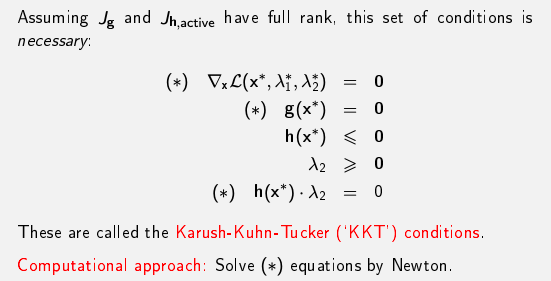
\includegraphics[width=\textwidth,height=\textheight,keepaspectratio]{lecture20_kkt}
\end{center}

Assemble the problem's inequalities as well as the complentarity condition for $h_i$ and the fact that $\lambda_2 \geq 0$ to obtain the KKT conditions listed above.



\end{document}





